\documentclass[twocolumn, amsmath]{revtex4}


\usepackage{graphicx}


\begin{document}


\title{PHYS 605 Lab\#2} 

\author{Evin O'Shea}  % fill in your name here
\author{Morgan Daly}
\email{eco2000@unh.edu}  % add your email address 
\date{\today}  


\begin{abstract}

	

\end{abstract}

\maketitle

%
%  Now that the initial formatting and first-page details are set, let's add some relevant sections to the paper
%
\section{Background}
The goal of Part 1 of the lab was to make current and voltage measurements of different circuit elements in order to characterize their current-voltage relationships. After taking measurements, the current and voltage can be plotted. This will give insight to the current-voltage relationship and will give the resistance of the elements. Lastly, the group needed to plot the power and voltage to investigate the power the elements dissipate.

The goal of Part 2 of the lab was to construct an R-2R ladder of resistors. The lab was designed to measure the equivalent resistance of the circuit through current and voltage measurements. Finding the equivalent resistance of the ladder as it is built will show how the ladder functions. Then the group was to find the Th\`{e}venin equivalent of an R-2R ladder to further investigate the nature of the circuit.


\section{Methodology}
For the first part of the lab, the group had to construct a circuit which would test the current-voltage relationships of various passive circuit components. The way this was done was by setting up a circuit in which a battery with adjustable voltage was connected to a resistor. Then the element was be placed in series with the resistor. Then a voltmeter was set up in parallel with the variable circuit element to measure the voltage drop across the element. Lastly, an ameter was connected in series with the battery to measure the total current of the circuit. Since the voltmeter has such a high resistance compared to the elements being used, it does not affect the current flow in the circuit. This means current flow that is measured by the ameter will be equal to the current flow through the elements used in the circuit. These measurements will be plotted to give the current-voltage relationships of the different circuit elements. Then the power can be calculated and can be plotted against voltage to show how the power dissipated relates to the voltage through the element. The power can be calculated using the equation below:

\begin{equation}
P = I^2R 
\end{equation}


For the second part of the lab, the group simply had to build an R-2R ladder and measure the equivalent resistance of the circuit as is was built. This was done by building the ladder in steps. The group only had 10k$\Omega$ resistors, which will be refered to as R in this section. To make 2R resistors, the group simply connected two 10k$\Omega$ resistors in series. The first step in building the circuit was to set up the voltmeter and ameter that would make the measurements of the circuit. The voltmeter was connected to the battery and was in parallel with the rest of the circuit at all times. This meant that the voltage of the battery would be measured by the voltmeter at all times. An ameter was set up in series between the ladder and the battery so that the total current of the circuit could be measured. These current and voltage measurments could be used with a form of Ohm's law to find the equivalent resistance of the circuit as shown below:

\begin{equation}
V = IR \implies R = \frac{V}{I}
\end{equation}

Next, the circuit was built in parts and the measurements were recorded as the parts were built. The first part built was made with just a 2R resistor. This would have a resistance of simply 2R or 20k$\Omega$. This circuit is shown below:

\begin{figure}[h]  

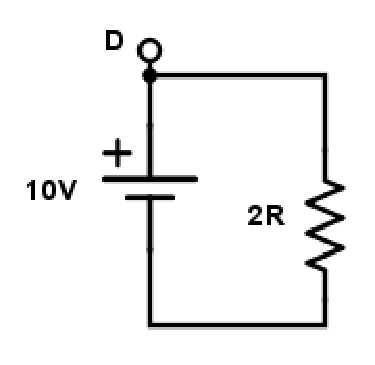
\includegraphics[scale = 0.4]{D.eps}  
\end{figure}

The ladder was then extended by adding a 2R resistor in parallel with the initial 2R resistor and a single R resistor added in series with the two 2R resistors that were in parallel. This circuit is shown below:

\begin{figure}[h]  

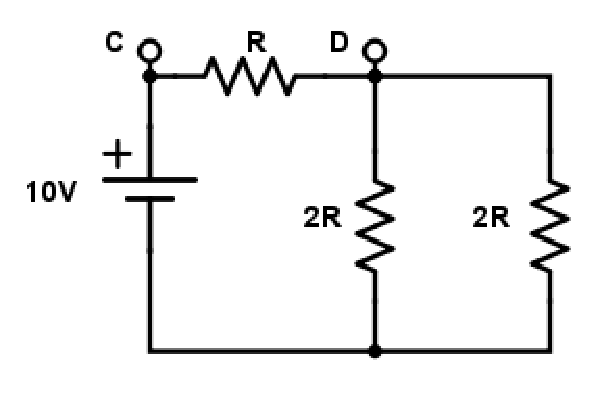
\includegraphics[scale = 0.4]{C.eps}  
\end{figure}

The equivalent resistance can be calculated by knowing that resistors in series add together and the equivalent resistance of resistors in parallel are given by the equation:
\begin{equation}
R_{parallel} = (\frac{1}{R_1}+\frac{1}{R_2})^{-1}
\end{equation}

The equaivalent resistance of this circuit would be calculated first by finding the resistance of the two 2R resistors in parallel:
$R_{parallel} = (\frac{1}{2R}+\frac{1}{2R})^{-1} = R$
and then adding this resistance to the single R resistor in series. The equivalent resistance of this piece of the ladder would simply be $R_{eq} = 2R$.

The group now just needed to repeat the last step of adding a 2R resistor in parallel with the part of the ladder that had already been created and adding a single R resistor in series with that. This part of the lab was repeated twice to obtain the circuit shown below:

\begin{figure}[h]  

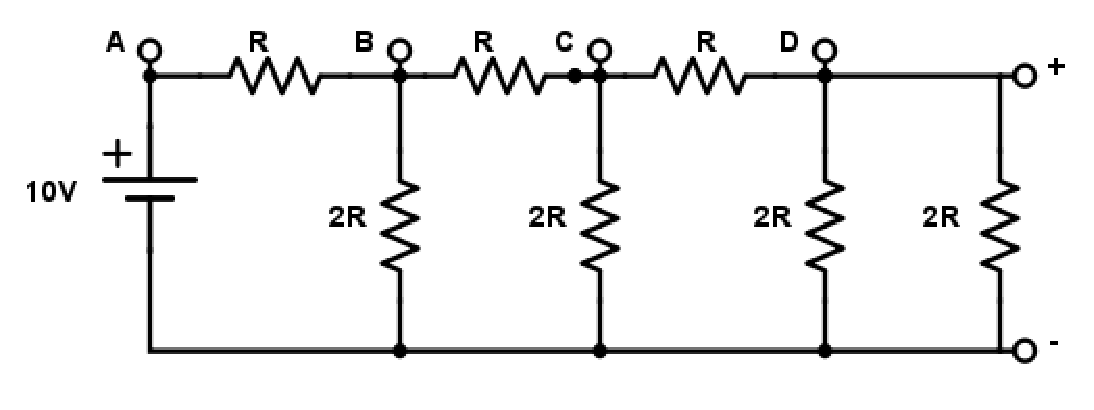
\includegraphics[scale = 0.4]{a.eps}  
\end{figure}

The voltage and current were measured each time the combination of an R and a 2R were added. Each time, the equivalent resistance should not change. This is becasue, as with the second measurement, the 2R elements in parallel will combine to an equivalent resistance of R and then will be added to the R that is in series with them. Each time a 2R is added in parallel, the previously built element will combine with the 2R component to create an equivalent resistance of R and then the R resistor that is in series will be added to create an equivalent resistance of 2R. The R-2R ladder should have a total equivalent resistance of 2R no matter how long the ladder is.

The last part of the lab was to find the Th\`{e}venin equivalent of a ladder. The ladder built was the one set of R-2R resistors more than the original ladder. The Th\`{e}venin equivalent is found by measuring the open circuit voltage and the short circuit current across the terminals labeled in the picture of the full ladder. This is done by connecting a voltmeter and an ameter in these locations at separate times. The measurements taken will be the Th\`{e}venin voltage, $V_{th}$, and the Norton current, $I_N$. These can be used to find the Th\`{e}venin resistance, $R_{th}$ by using equation (2).

\section{Results and Analysis}
The circuit designed for this part of the lab is shown below:

\begin{figure}[h]  

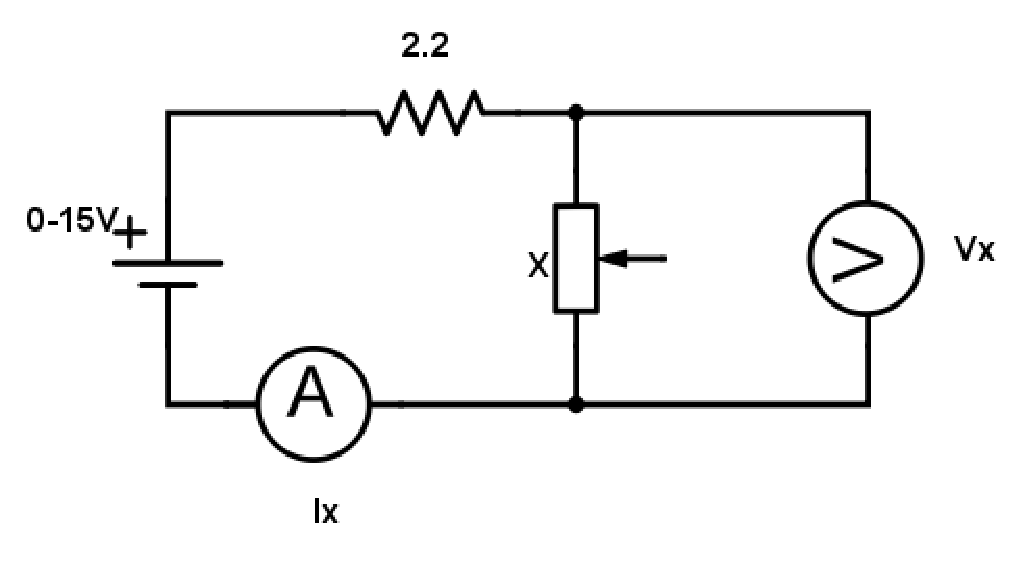
\includegraphics[scale = 0.4]{par1.eps}  
\caption{The resistor has a value of 2.2k$\Omega$}
\end{figure}

For each element, measurements were made by adjusting the voltage of the battery in the circuit and recording the measurements made by the voltmeter and ameter. The data recorded for the first part of the lab will be shown below in a table and in a graph. The slopes of the current-voltage graphs is $\frac{1}{R}$ as given from equation (2).


For the 47$\Omega$ resistor the measurements were:

\begin{center}
    \begin{tabular}{| l | l | l | l |}
    \hline
    $V_{o} (V)$ & $V_{X} (mV)$  & $I_{X} (mA)$ & $P (nW)$ \\ \hline
    
    1.263	& 26.1  	& 0.56  &   14.6	 \\ \hline
    2.586	& 53.5  	& 1.14 	 &  61.0	\\ \hline
    4.12	& 85.7  	& 1.83	 &  157	\\ \hline
    7.22    	& 150.5  	& 3.21  &  483	 \\ \hline
    8.88   	& 185.0    	& 3.95  &   731	 	\\ 
    \hline
    \end{tabular}
\end{center}

The current-voltage relationship is splotted below:
	
\begin{figure}[h]  

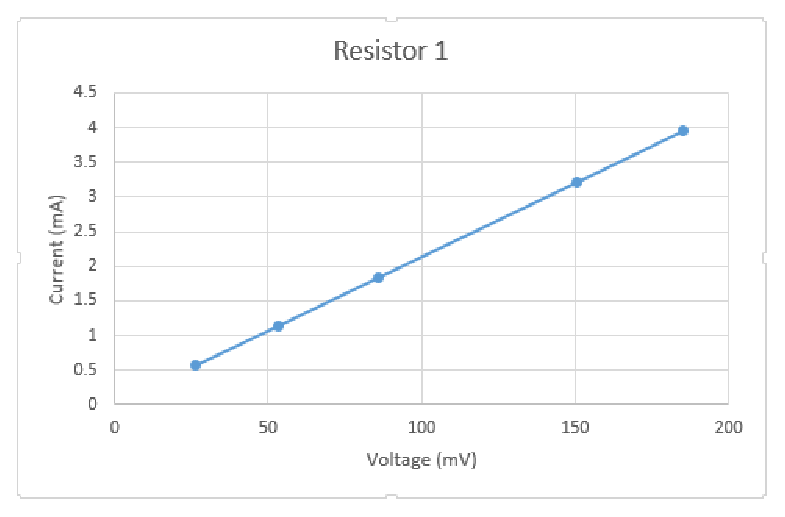
\includegraphics[scale = 0.4]{Resistor.eps}  
\end{figure}

The data recorded and plotted demonstrate an accurate current-voltage relation for a resistor as there is a stright line with positive slope. This slope is constant shows that the current-voltage relationship for a resistor is linear. This means that the resistance is constant with varying voltage.

The plot of voltage and power for the 47$\Omega$ resistor is shown below:

\begin{figure}[h]  

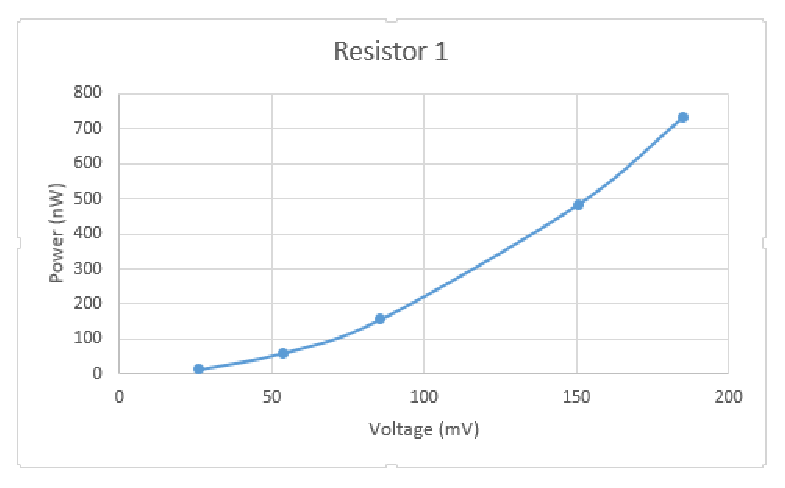
\includegraphics[scale = 0.4]{powerresistor.eps}  
\end{figure}

This plot is non-linear because power depends on the square of the current as shown in equation (1). Since R is constant, changing the voltage changes the current. This means that the power will change proportionally to the square of the voltage as the voltage is varied. This explains the quadratic nature of the graph.


For Diode 1 the measurements were:

\begin{center}
    \begin{tabular}{| l | l | l | l |}
    \hline
    $V_{o} (V)$ & $V_{X} (V)$ & $I_{X} (mA)$ & $P (mW)$ \\ \hline
    
    1.261	& 0.535  	& 0.32  & 0.171 	 \\ \hline
    2.784	& 0.588  	& 0.99 	& 0.582	\\ \hline
    6.61	& 0.635  	& 2.70	& 1.71   \\ \hline
    11.44    	& 0.661  	& 4.90  & 3.24 	 \\ \hline
    14.55   	& 0.672    	& 6.32  & 4.25 	 	\\ 
    \hline
    \end{tabular}
\end{center}

The current-voltage relationship is splotted below:
\vspace{.8cm}	
\begin{figure}[h]  
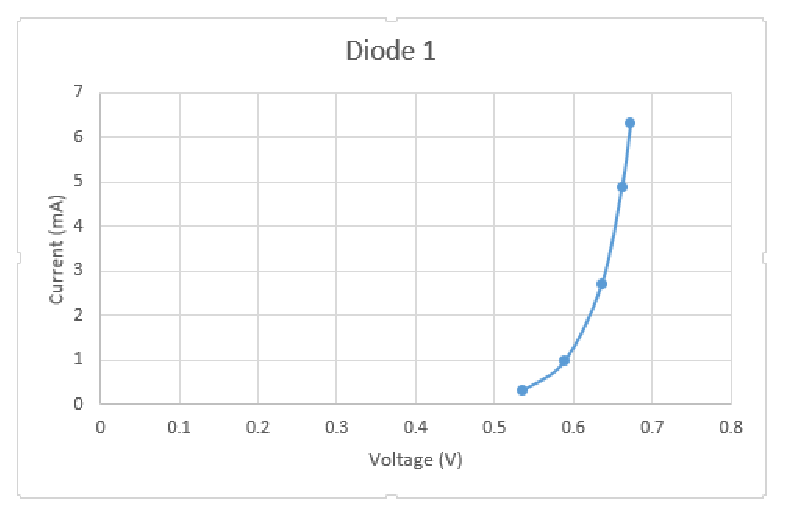
\includegraphics[scale = 0.4]{Diode1.eps}  
\end{figure}
The plot of voltage and power for Diode 1 is shown below:

\begin{figure}[h]  

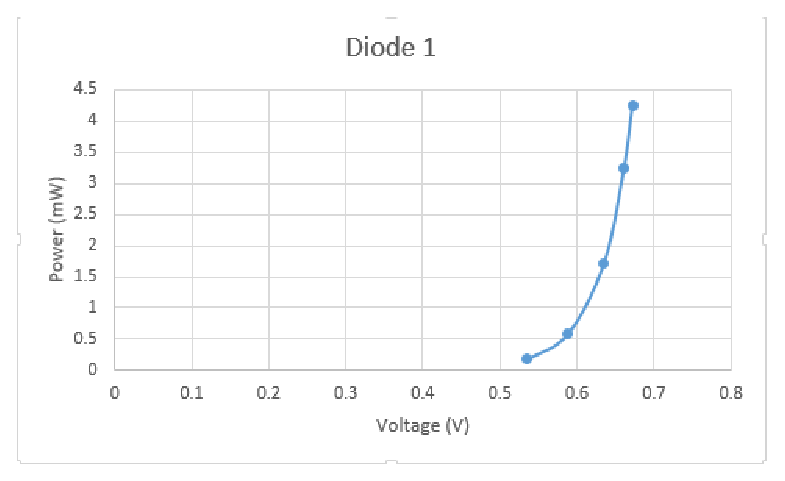
\includegraphics[scale = 0.4]{powerdiode1.eps}  
\end{figure}

For Diode 2 the measurements were:

\begin{center}
    \begin{tabular}{| l | l | l | l |}
    \hline
    $V_{o} (V)$ & $V_{X} (V)$  & $I_{X} (mA)$ & $P (mW)$ \\ \hline
    
    1.261	& 0.537  	& 0.32  & 0.172	 \\ \hline
    3.766	& 0.606  	& 1.42 	& 0.861	\\ \hline
    7.70	& 0.643  	& 3.19	& 2.05	\\ \hline
    11.26    	& 0.661  	& 4.81  & 3.18	 \\ \hline
    14.93   	& 0.674    	& 6.49  & 4.37	 	\\ 
    \hline
    \end{tabular}
\end{center}


The current-voltage relationship is splotted below:
	
\begin{figure}[h]  

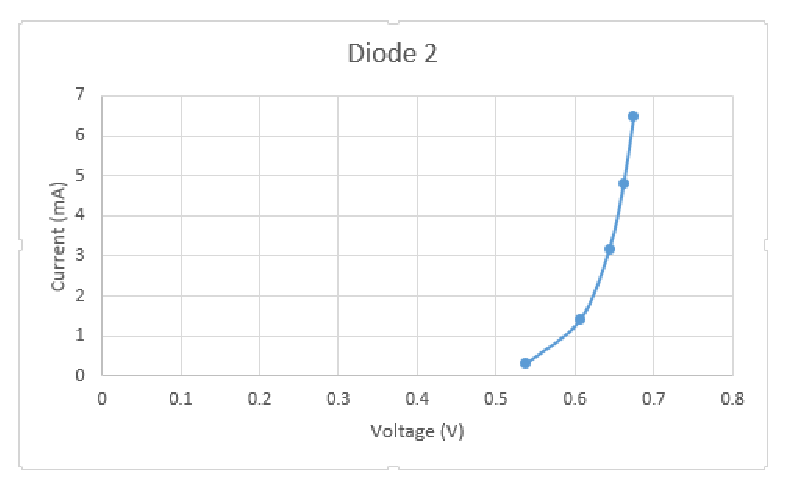
\includegraphics[scale = 0.4]{diode2new.eps}  
\end{figure} 

\newpage

The power-voltage relationship is shown below:

\begin{figure}[h]  

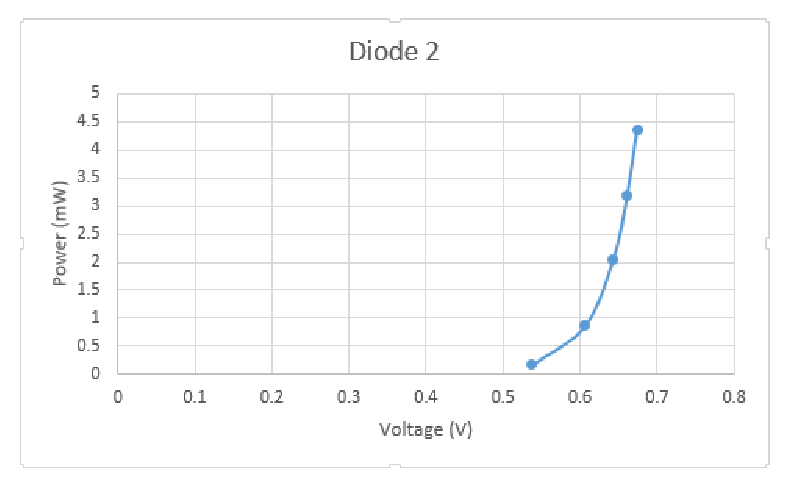
\includegraphics[scale = 0.4]{powerdiode2.eps}  
\end{figure}


The two diodes were of the same make and had similar current-voltage relationships. The plots show a non-linear current-voltage relationship. Since the slope is $\frac{1}{R}$ and the slope increases as voltage increases, the resistance of the diodes decreases as voltage increases. This gives the interesting current-voltage relationship shown. The power dissipated looks similar to the current-voltage graph. Since the resistance decreased as voltage increased, it made the current-voltage plot look exponential. Since power is related to the square of the current and the current changes non-linearly, the power-voltage plot will have a similar, non-linear, curve. 


\vspace{1cm}
For the zener diode the measurements were:
\begin{center}
    \begin{tabular}{| l | l | l | l |}
    \hline
    $V_{o} (V)$ & $V_{X} (V)$  & $I_{X} (mA)$ & $P (mW)$ \\ \hline
    
    2.171	& 0.704  	& 0.66  & 0.465 	 \\ \hline
    5.14	& 0.735  	& 1.99 	& 1.46	\\ \hline
    8.24	& 0.750  	& 3.41	& 2.56 	\\ \hline
    12.05    	& 0.760  	& 5.13  & 3.90	 \\ \hline
    14.81   	& 0.767    	& 6.40  & 4.91	 	\\ 
    \hline
    \end{tabular}
\end{center}

The current-voltage relationship is splotted below:
	
\begin{figure}[h]  

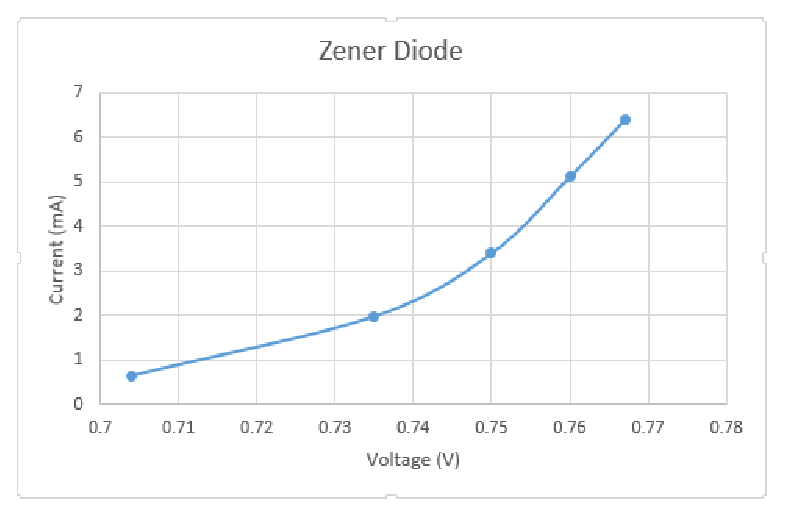
\includegraphics[scale = 0.4]{zenerdiode.eps}  
\end{figure}

The power dissipated versus voltage plot for the zener diode is shown below:

\begin{figure}[h]  

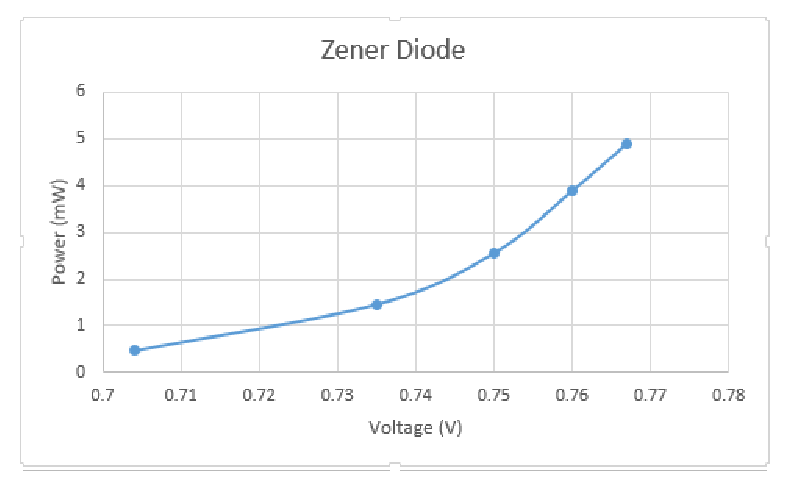
\includegraphics[scale = 0.4]{powerzener.eps}  
\end{figure}

\newpage

For the light emitting diode the measurements were:

\begin{center}
    \begin{tabular}{| l | l | l | l|}
    \hline
    $V_{o} (V)$ & $V_{X} (V)$  & $I_{X} (mA)$ & $P (mW)$ \\ \hline
    
    4.64	& 1.670  	& 1.35		& 2.25 	 \\ \hline
    6.63	& 1.698  	& 2.24 	 	& 3.80	\\ \hline
    8.04	& 1.713  	& 2.87	 	& 4.92	\\ \hline
    10.57    	& 1.735  	& 4.01  	& 6.96	 \\ \hline
    13.84   	& 1.758    	& 5.50  	& 9.67	 	\\ 
    \hline
    \end{tabular}
\end{center}

The current-voltage relationship is splotted below:
	
\begin{figure}[h]  
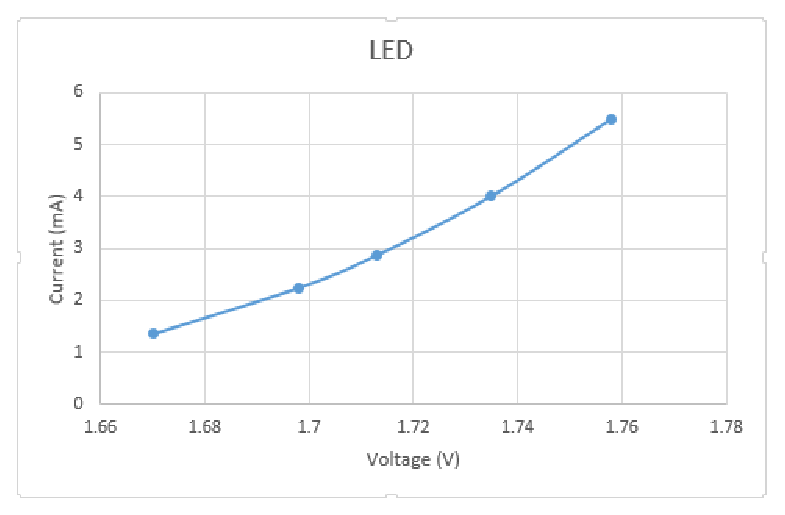
\includegraphics[scale = 0.4]{LED.eps}  
\end{figure}

The power-voltage plot for the LED is shown below:

\begin{figure}[h]  

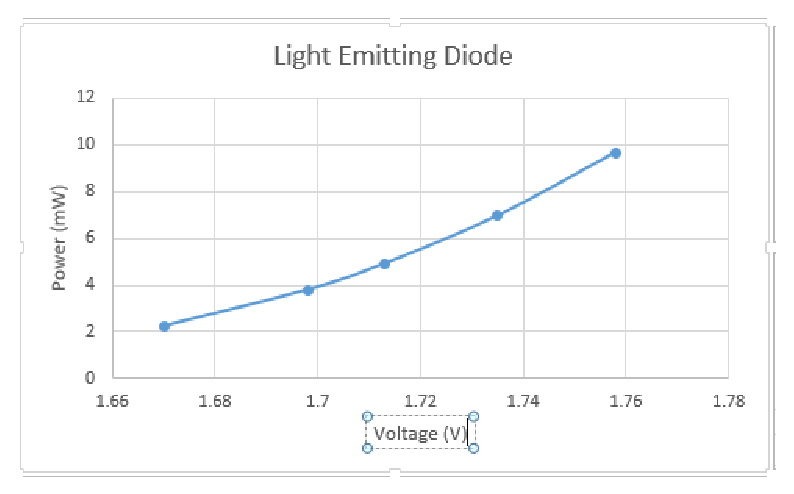
\includegraphics[scale = 0.4]{powerled.eps}  
\end{figure}

For both the zener diode and the light emitting diode, the current-voltage relationship was similar to the plain diodes. As voltage increased the slope increased. This means that the resistance decreased as voltage increased for the light emitting diode and the zener diode as well as the regular diodes. This has a similar affect on the power-voltage plot as it did for the plain diodes. The other diodes had a non-linear curves that looked similar for both plots. For the LED and the zener diodes, this was also the case. 

The diodes were placed in the circuit in the reverse direction and no current flowed through. This is because diodes only let current flow in one direction. When in the wrong direction, no current will flow through the diode and for the LED it will not light up.





For the second part of the lab, thr group had to build an R-2R ladder piece by piece and measure the total voltage and total current of the circuit to measure the equivalent resistance of each peice of the circuit. All of the values of the resistors were measured and only one was outside of the tolerance range. The values measured will be used in all calculations of expected resistances. The combined ladder and all resistors used are shown:

\newpage

\begin{figure}[h]  

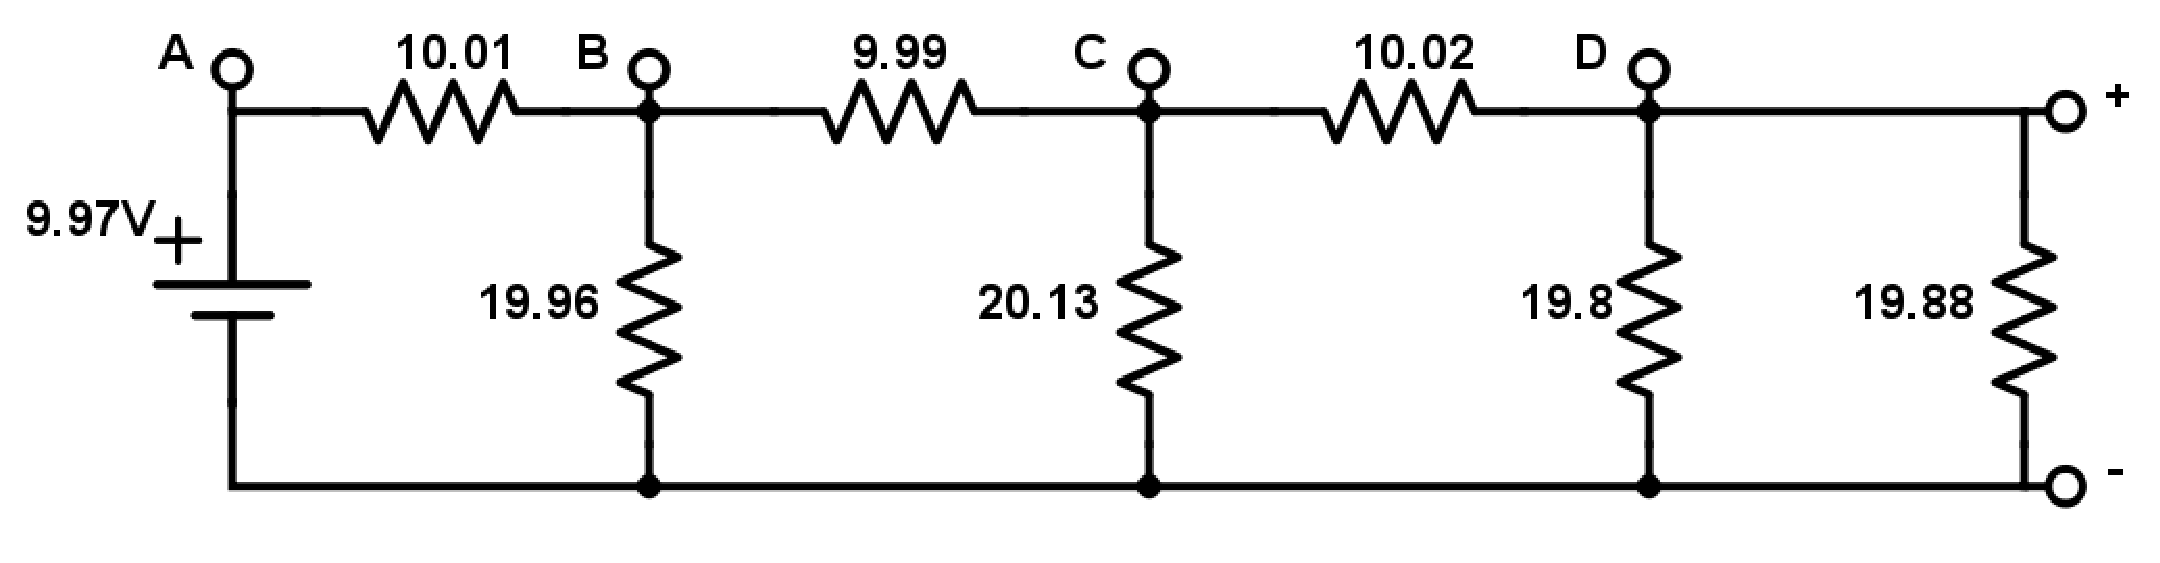
\includegraphics[scale = 0.23]{valuesA.eps}  
\caption{All resistances labeled are in k$\Omega$}
\end{figure}



\begin{center}
    \begin{tabular}{| l | l | l | l | l | l|}
    \hline
    $Terminal$ & $V_o (V)$  & $I_{total} (mA)$ & $R_{eq} k\Omega$ & $R_{expected} k\Omega$ & \% Error \\ \hline
    D		& 9.97		& 0.49 		& 20.34		& 19.88 	& 2.31 			  \\ \hline
    C		& 9.97  	& 0.50 		& 19.94		& 19.94		& >0.01			 \\ \hline
    B		& 9.97	 	& 0.50		& 19.94		& 20.01		& 0.336			 \\ \hline
    A   	& 9.97	 	& 0.50  	& 19.94		& 20.00 	& 0.312 		\\ 
    \hline
    \end{tabular}
\end{center}

The calculated values for $R_{expected}$ were obtained using the circuit combinations methods described in the Methodology section. These calculated values are well reflected by the measured data and the low percent error values.  This demonstrates the R-2R ladder's functionality as the equivalent resistance is approximately 2R in all cases. More can be uncovered about the utility of the R-2R ladder by examining the Th\`{e}venin equivalent of the circuit. To find Th\`{e}venin equivalent of an R-2R ladder, the group built the ladder shown below:

\begin{figure}[h]  

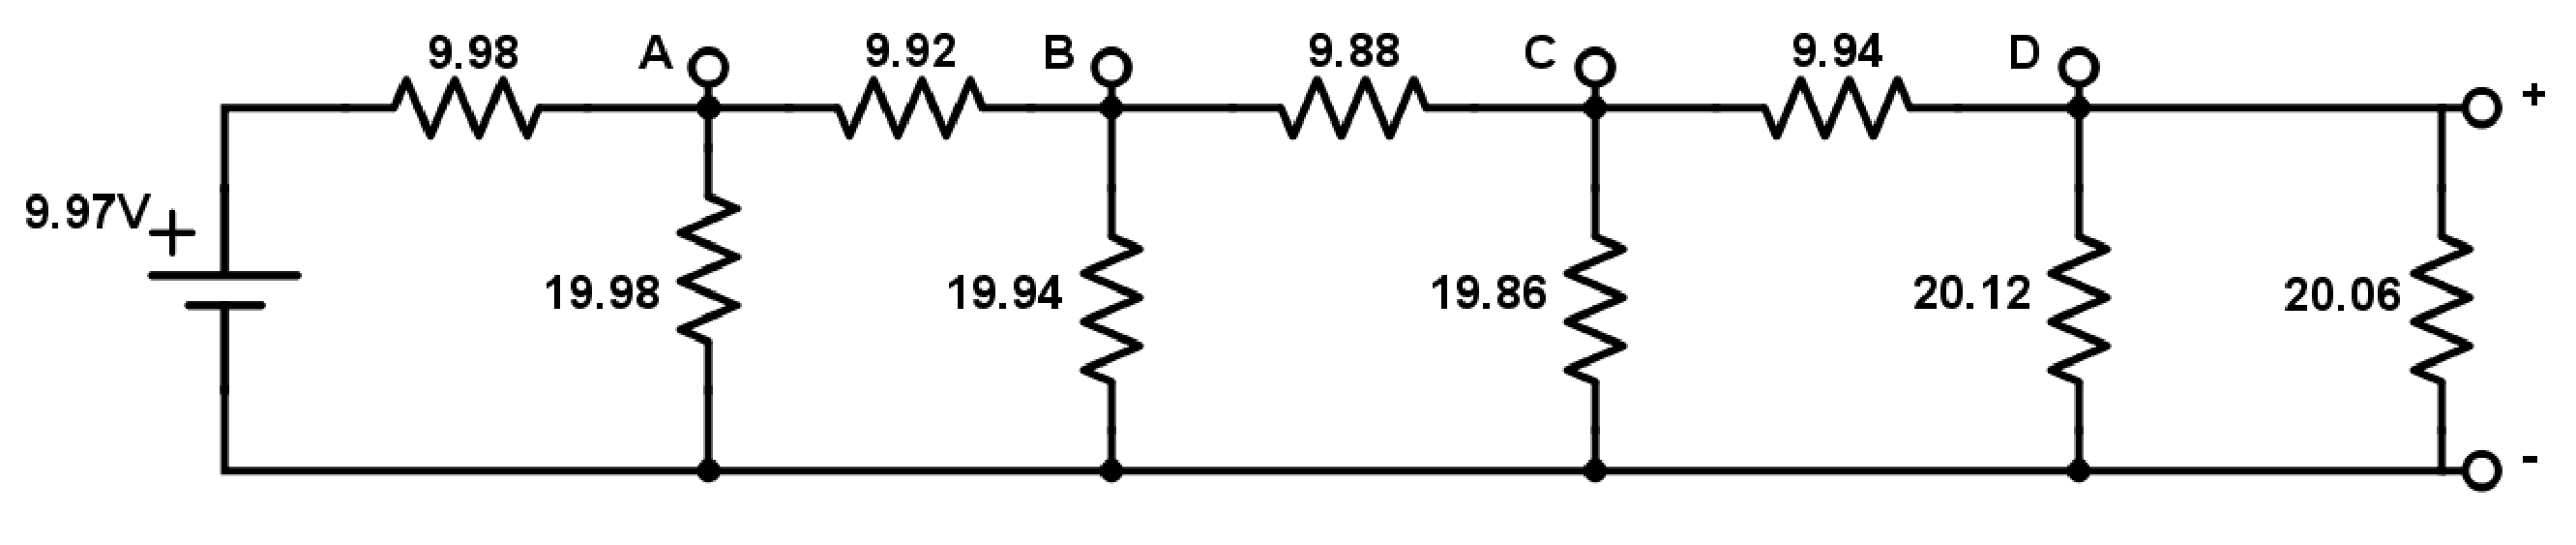
\includegraphics[scale = 0.2]{ladderthevenin.eps}  

\end{figure}

The Th\`{e}venin equivalent gives knowledge about how the circuit will work when a source is attatched to the + and - terminals of the ladder. The Th\`{e}venin equivalent is found by finding the open-circuit voltage across the terminals this was measured to be $V_{th} = 0.636V$. The Th\`{e}venin resistance is found by finding the norton current and using equation (2) to calculate $R_{th}$. The current was measured to be $I_N = 88.8\mu A$. This means that the Th\`{e}venin resistance would be $R_{th} = 3.58k\Omega$.

The Th\`{e}venin equivalent circuit is shown below:

\begin{figure}[h]  

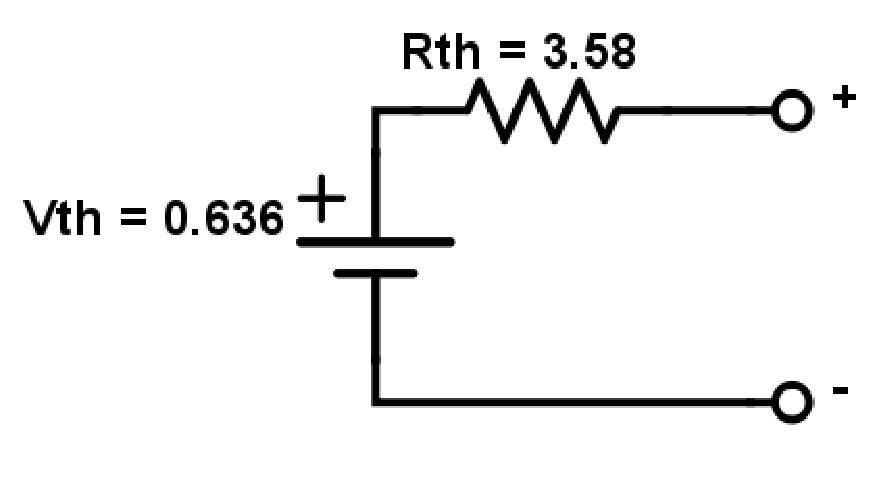
\includegraphics[scale = 0.4]{theveq.eps}  

\end{figure}


This demonstrates, that the ladder not only has an equivalent resistance of just 2R, but also has split the voltage from 9.97V to 0.636V. This means the output voltage is approximately $\frac{1}{16}$ the input voltage. The ladder splits voltage affectively, as the output voltage can easily be controlled.

\newpage

\section{Conclusion}

The first part of the lab was to examine the current-voltage relationships of multiple passive circuit elements. This was dones successfully as the group examined a resistor and various types of diodes. These different elements had interesting current volateg relationships. For the resistor, as expected, the resistance did not change with voltage. For the diodes, all of them showed a decrease in resistance as the voltage source was increased. The power dissipated and voltage were also graphed for all of these elements. Similar results were shown about the power output and how it changes with the voltage source; however, the resistor had a linear relationship for the current-voltage plot and a quadratic nature for power-voltage. This is expected as power is proportional to the square of the voltage.

\vspace{.8cm}

For the second part of the lab the group was to construct an R-2R ladder and to measure the equivalent resistance as multiple parts were built. The group did this successfully as the results were varified by calculations to be within reasonable accuracy. This demonstrated that the R-2R ladder has an equivalent resistance of 2R no matter how long it is. The last part of the lab was to find the Th\`{e}venin equivalent of an R-2R ladder. This was also done successfully as the output voltage of the ladder was as expected. This demonstrated how the ladder split the voltage multiple times giving an output voltage that was only a fraction of the input voltage.


\end{document}
